\documentclass[a4paper]{article}  

\usepackage{amsmath}
\usepackage{tikz}
\usepackage{algpseudocode}

\title{CS270 Homework 1}
\author{Valkyrie Savage}

\begin{document}
\maketitle

\begin{enumerate}
\item Short answers
	\begin{enumerate}
	\item An asymptotically tight upper bound on the recurrence $T_1 = 4T_1 (n/3) + O(n^2 ), T_1 (1) = O(1)$ is $O(n^2 )$.  For the recurrence $T_2 (n) - 27T_2 (n/3) + O(n^2 ), T_2 (1) = O(1)$, we also have the bound $O(n^2 )$.
	\item She can multiply $4x4$ matrices in 32 scalar multiplies ($2n^2$) and 67 additions and subtractions ($n^3+3$).  This means that the operation is $O(n^3 )$.
	\item Given an edge $e$ contained in the minimum cut of a max flow problem, by increasing the capacity of $e$ we don't necessarily increase the maximum flow.  The \textbf{max-flow min-cut theorem} states that the size of the maximum flow in a network equals the capacity of the smallest $(s,t)$ cut, however as a counterexample consider a network
		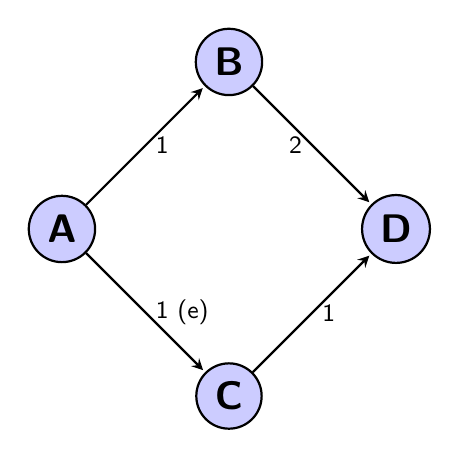
\begin{tikzpicture}[->,>=stealth,shorten >=1pt,auto,node distance=3cm,
 		thick,main node/.style={circle,fill=blue!20,draw,font=\sffamily\Large\bfseries}]

  		\node[main node] (B) {B};
  		\node[main node] (A) [below left of=B] {A};
  		\node[main node] (C) [below right of=A] {C};
  		\node[main node] (D) [below right of=B] {D};

  		\path[every node/.style={font=\sffamily\small}]
    		(B) edge node [left] {2} (D)
    		(A) edge node [right] {1} (B)
        		edge node [right]  {1 (e)} (C)
    		(C) edge node [right] {1} (D);
		\end{tikzpicture}\\
		With edge $e$ as noted (connecting A to C), then $e$ can be part of a min cut.  The max flow of the system is currently 2.  However, if we increase $c(e)$ to 2, then the max flow of the system is still 2, and $e$ is no longer part of a min cut.
	\item $max min(x+y,y+w,3x+w)\\x+y+w=1$
	\item 
	\item
	\item
	\end{enumerate}
\item Point domination
	\begin{enumerate}
	\item An efficient algorithm to find all points of set $S$ which do not dominate any other point in $S$:
	\item An efficient algorithm to find the largest subset of points $U$ where for each pair of points in $U$ neither dominates the other:
	\end{enumerate}
\item Clauses
\item Pattern Subsequences
	\begin{enumerate}
	\item An $O(nm)$ algorithm for finding any occurrence of $s_1$ within $s_2$ with $k$ or fewer mismatched bits:\\
		\begin{algorithmic}
		\State $matchlocations \gets [ ]$
		\State $i \gets 0$
		\For{$i < n$}
			\State $count \gets 0$
			\State $j \gets 0$
			\For{$j < m$}
				\If {$s_2[i+j] != s_1[j]$}
					\State $count++$
				\EndIf
				\State $j \gets j + 1$
			\EndFor
			\If {$count < k$}
				\State $matchlocations \gets (matchlocations, i)$
			\EndIf
			\State $i \gets i + 1$
		\EndFor
		\State return $matchlocations$
		\end{algorithmic}
	\item An $O(n log n)$ algorithm for any k:
		\begin{algorithmic}
		\State $matchlocations \gets [ ]$
		
		\State return $matchlocations$
		\end{algorithmic}
	\end{enumerate}
\item Sorting by Reversals
	\begin{enumerate}
	\item
	\item
	\end{enumerate}
\end{enumerate}
\end{document}